\documentclass{article}
\usepackage[utf8]{inputenc}
\usepackage[T1]{fontenc}
\usepackage[german]{babel}
\usepackage{amsmath}
\usepackage{amsthm}
\usepackage{amsfonts}
\usepackage{amssymb}
\usepackage{minted}
\usepackage{tikz}
\usepackage{pgfplots}
\usepackage[top=2cm, bottom=2cm, left=2cm, right=2cm, headheight=1.5cm]{geometry}
\usepackage{fancyhdr}
\usepackage{mdframed}
\usemintedstyle{emacs}

\definecolor{purp}{HTML}{9A72AC}
\definecolor{re}{HTML}{FC6255}
\definecolor{gre}{HTML}{83C167}
\definecolor{blu}{HTML}{58C4DD}
\definecolor{shadecolor}{rgb}{0.85,0.85,0.85}
\definecolor{bg}{rgb}{0.95,0.95,0.95}
\setlength{\parindent}{0em} 

\BeforeBeginEnvironment{minted}{\begin{mdframed}[linewidth =2 ,backgroundcolor=bg , linecolor=black, linewidth=0.5]}
\AfterEndEnvironment{minted}{\end{mdframed}}

\newenvironment{defi}[1]{
    \begin{shaded*}
    \textbf{Definition #1} \\
}{
    \end{shaded*}
}

\newcommand{\bsp}{\textbf{Beispiel}:}
%\newcommand{\task}{\textbf{Aufgabe}:}

\newcommand{\bol}[1]{\textbf{#1}}
\newcommand{\q}[1]{\glqq #1\grqq}
\newcommand{\DODO}[1]{\textbf{\textcolor{red}{DODO:}} #1 \\ \begin{center}\includegraphics[scale=0.2]{../../media/dodo.jpg} \end{center}}

\newenvironment{task}[1]{
    \begin{shaded*}
    \textbf{Aufgabe #1}:
}{
    \end{shaded*}
}



\fancypagestyle{firstpage}{
    \setlength{\headheight}{2.5cm}
    \setlength{\footskip}{0.25cm}
    \pagestyle{fancy}
    \renewcommand{\headrulewidth}{0.4pt}
    \fancyhf{}
    \fancyhead[L]{\LARGE\textbf{Musterlösung und Erläuterungen S. 218|3}}
    \fancyfoot[C]{\thepage}
}
\begin{document}
\thispagestyle{firstpage}
\setlength{\headsep}{12pt}
Aufgabentext:
\begin{center}
    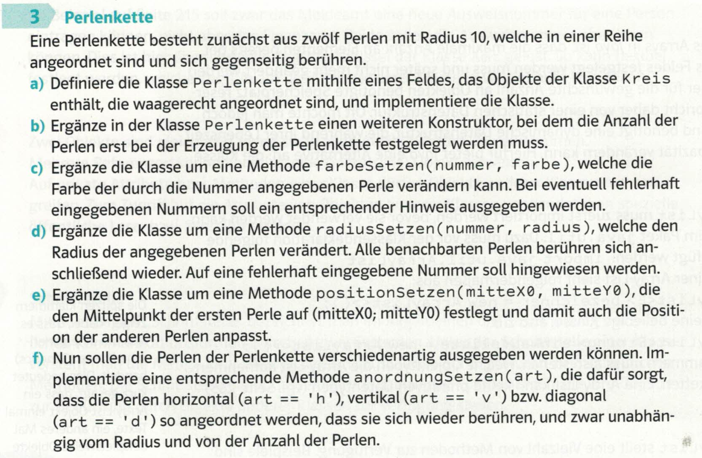
\includegraphics[scale=0.6]{media/218_3.png}
\end{center}
Wie bereits im Unterricht besprochen besteht eine Perlenkette in der ersten Teilaufgabe aus zwölf Kreisen, d.h. unsere Klasse benötigt als Attribut ein Array von Kreis-Objekten. Da in Teilaufgabe b) noch ein zweiter Konstruktor gebaut werden soll, wird das Array erst im Konstruktor initialisiert. Dort muss es danach noch mit Kreisen gefüllt werden, die in einem ersten Schritt einen Radius von 10 haben:
\begin{minted}{java}
public class Perlenkette {
    //Das Kreis-Array wird als Attribut der Klasse Perlenkette definiert
    private Kreis[] perlen;

    //a) Der Konstruktor soll zwölf Perlen mit Radius 10 erzeugen:
    public Perlenkette() {
        //Das Array wird initialisiert
        perlen = new Kreis[12];
        //Das Array wird durchlaufen...
        for(int i = 0; i < perlen.length; i++) {
            //und an jeder Stelle des Arrays wird ein neuer Kreis gespeichert
            //Der Konstruktor eines Kreises nimmt als Eingabeparameter den Radius
            perlen[i] = new Kreis(10);
            //Jetzt müssen die Perlen noch abhängig von ihrer Position in der Kette
            //verschoben werden, dazu wird die "verschieben"-Methode der einzelnen 
            //Kreise verwendet
            perlen[i].verschieben(2*10*i,0);
            //die i-te Kugel muss dabei um i*Durchmesser einer Kugel verschoben werden
        }
    }
}
\end{minted}
Teilaufgabe b) ist deutlich einfacher, es muss nur Teilaufgabe a) kopiert werden und ein Eingabeparameter verwendet werden (im Folgenden werden immer nur die neuen Methoden abgebildet):
\begin{minted}{java}
//b)
public Perlenkette(int anzahl) {
    //Die relevante Änderung, das Array wird so groß wie gewünscht erzeugt
    //Nicht gefordert in der Aufgabenstellung, aber sinnvoll: 
    //eine Überprüfung, ob die Eingabe sinnvoll ist! 
    //Wenn die Anzahl kleiner oder gleich 0 ist...
    if(anzahl <= 0) {
        //... wird die Anzahl auf 5 festgelegt-
        anzahl = 5;
    }
    perlen = new Kreis[anzahl];
    for(int i = 0; i < perlen.length;i++) {
        perlen[i] = new Kreis(10);
        perlen[i].verschieben(2*10*i, 0);
    }
}
\end{minted}
Für Teilaufgabe c) ist wichtig, dass nicht immer das gesamte Array durchlaufen werden muss. Mit der []-Notation kann auf einzelne Elemente zugegriffen werden. \\
\textbf{Erinnerung:}
\begin{center}
    Wenn das Array \textit{zahlen} $= \{5,3,7,8\}$gegeben ist, liefert \textit{zahlen}[1] den Wert $3$ 
\end{center}
Damit zur Lösung (Man könnte noch eine Überprüfung einbauen, ob eine korrekte Farbe eingegeben wurde):
\begin{minted}{java}
//c)
public void farbeSetzen(int nummer, String farbe) {
    //zunächst wird geprüft, ob die eingegeben Zahl innerhalb der Feldgrenzen liegt
    if(nummer < 0 || nummer >= perlen.length) {
        System.out.println("Diese Perle gibt es nicht!");
        //falls nicht wird eine Meldung ausgegeben und beendet!
        return;
    }
    //Andernfalls wird die Perle (der Kreis) an der Stelle "nummer" mit Hilfe der
    //Kreis-Methode farbeSetzen (deswegen Punktnotation!) auf die übergebene
    //Farbe gesetzt
    perlen[nummer].farbeSetzen(farbe);
}
\end{minted}

Die Teilaufgabe d) beginnt ähnlich wie Teilaufgabe c) (wir überprüfen die korrekte Eingabe), aber für die Verschiebung muss noch einiges an Überlegung angestellt werden:
\begin{minted}{java}
//d)
public void radiusSetzen(int nummer, double radius) {
    if(radius <= 0) {
        System.out.println("Der Radius ist zu klein!");
        return;
    }
    //Wir speichern den alten Radius der Kugel in einer Variable (also einer Art) 
    //"Zwischenspeicher" ab, dazu verwenden wir die radiusGeben()-Methode des Kreises
    double alterRadius = perlen[nummer].radiusGeben();
    //Dann verschieben wir zuerst die vergrößerte (verkleinerte) Perle:
    perlen[nummer].verschieben(radius-alterRadius, 0);
    //Wir verwenden hier die Differenz, da der Kreis nicht seinen neuen Radius weiterwandert,
    //sondern nur den Wert, um den er größer bzw. kleiner geworden ist. 
    //Danach müssen noch alle anderen Perlen angepasst werden, außer wir haben die 
    //letzte Perle vergrößert (Spezialfall!):
    if(nummer == perlen.length - 1) {
        //In diesem Fall sind wir fertig und können abbrechen
        return;
    }
    //Andernfalls verschieben wir ab der Perle "nummer + 1", wollen wir also z.B.
    //die fünfte Perle von 10 verschieben, müssen die Perlen 6 bis 10 verschoben werden.
    for(int i = nummer + 1; i < perlen.length; i++) {
        //Es muss wieder um die Differenz verschoben werden, aber diesmal zweimal
        //(da der Kreis ja auf beiden Seiten um die Differenz geschrumpft bzw
        //gewachsen ist!)
        perlen[i].verschieben(2*(radius-alterRadius),0);
    }
}
\end{minted}
Für die Teilaufgabe e) muss beachtet werden, dass die einzelnen Kreise \q{nachgezogen} werden müssen. Die einfachste Methode das zu realisieren ist, den Mittelpunkt des ersten Kreises zu setzen, und die Mittelpunkte der anderen Kreise relativ zu ihm neu zu setzen. Alternativ können auch alle Kreise auf dieselbe Position gebracht werden und dann wieder nach rechts geschoben werden, das wäre hier aber schwerer möglich als im Konstruktor, da die einzelnen Perlen bereits einen unterschiedlichen Radius haben können. 
\begin{minted}{java}
//e)
public void positionSetzen(double mitteX0, double mitteY0) {
    //Die erste Perle in der Reihe wird an die neue Position gesetzt
    perlen[0].mittelpunktSetzen(mitteX0, mitteY0);
    //Ab der zweiten Perle muss nachgezogen werden!
    for(int i = 1; i < perlen.length; i++) {
        //Für die jeweils i-te Perle (also perlen[i]) setzen wir den neuen Mittelpunkt,
        // indem wir uns von der  vorangehenden Perle (also perlen[i-1]) Informationen holen.
        //x-Richtung: Wir starten beim Mittelpunkt der vorangehenden Perle (mitteXGeben()) 
        //und laufen dann den Radius der vorangehenden Perle und dann den Radius
        //der aktuellen Perle
        //y-Richtung: Wir bleiben auf derselben Höhe, verwenden also einfach mitteY0
        //Für eine bessere Übersichtlichkeit ist der Methodenaufruf hier auf 
        //mehrere Zeilen verteilt
        perlen[i].mittelpunktSetzen(
            perlen[i-1].mitteXGeben() 
            + perlen[i-1].radiusGeben()
            + perlen[i].radiusGeben(),
            mitteY0
        );
    }
}
\end{minted}
Teilaufgabe f) ist relativ kompliziert bzw. zumindest aufwändig zu implementieren. Zunächst muss eine Fallunterscheidung getroffen werden, abhängig von der Art der Anordnung, müssen dann alle Perlen außer der ersten wieder mit mittelpunktSetzen() verschoben werden, nämlich nach rechts, nach unten oder nach \q{schräg} rechts unten. Wir gehen dabei von einem 45 Grad Winkel für \q{diagonal} aus:
\begin{minted}{java}
public void anordnungSetzen(char art) {
    //Fr die horizontale Anordnung...
    if(art == 'h') {
        //wird aber der zweiten perle verschoben
        for(int i = 1; i <perlen.length;i++) {
            //und zwar genauso wie in der vorangegabenen Methode!
            //Der einzige Unterschied: die y-Position der vorangehenden Perle
            //ist kein Eingabeparameter mehr, sondern muss geholt werden
                perlen[i].mittelpunktSetzen(
                perlen[i-1].mitteXGeben() 
                + perlen[i-1].radiusGeben() 
                + perlen[i].radiusGeben(),
                perlen[i-1].mitteYGeben()
            );
        }
    } else if(art == 'v') {
        //Für die vertikale Anordnung wird in y-Richtung, statt in x-Richtung verschoben
        //ansonsten ist alles analog
        for(int i = 1; i <perlen.length;i++) {
            perlen[i].mittelpunktSetzen(
                perlen[i-1].mitteXGeben(),
                perlen[i-1].mitteYGeben() 
                + perlen[i-1].radiusGeben()
                + perlen[i].radiusGeben()
            );
        }
    } else if(art == 'd') {
        //Für die Diagonale muss natürlich in beide Richtungen verschoben werden
        for(int i = 1; i <perlen.length;i++) {
            //Die eigentliche Verschiebung ist eigentlich ein mathematisches Problem
            //In diesem Fall brauchen wir natürlich wieder beide Radien, für eine
            //bessere Übersichtlichkeit speichern wir sie zwischen:
            double radiusAlt = perlen[i-1].radiusGeben();
            double radiusNeu = perlen[i].radiusGeben();
            //Überlegt man sich die Verschiebung geometrisch, so stellt man fest, 
            //dass eine Verschiebung um "Wurzel 2 geteilt durch 2" nötig wäre.
            //Für unsere Zwecke ist aber eine Näherung von 0,7 völlig ausreichend
            perlen[i].mittelpunktSetzen(
                perlen[i-1].mitteXGeben() + 0.7*(radiusAlt + radiusNeu),
                perlen[i-1].mitteYGeben() + 0.7*(radiusAlt + radiusNeu)
            );
        }
    } else {
        //Falls keine der Anordnungen passt wird einfach nichts gemacht!
        System.out.println("Die Anordnung ist nicht möglich");
    }
}
\end{minted}
\end{document}